% !TeX root = ../main.tex

\subsection{Measuring an f-I Curve}

Next, we used an oscilloscope to examine the neuron spiking frequency in response to different input currents. We measured the firing frequency of the Lu.i neuron for \num{20} different input currents (determined through the voltages).

After calculating the input current from the measured voltages, the \( f\) - \( I \) curve could be graphed in \autoref{fig:f-I_curve}.

\begin{figure}[htbp]
    \centering
    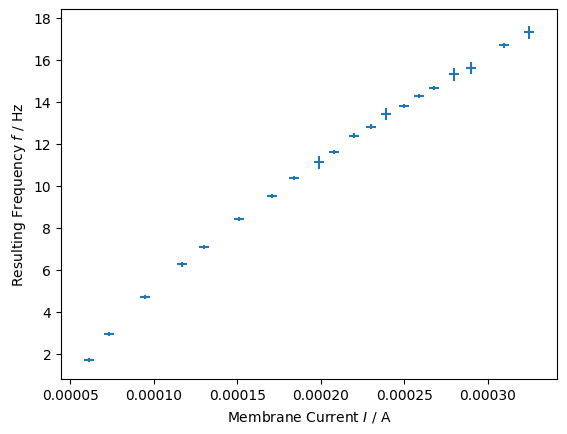
\includegraphics[width=0.7\textwidth]{./Experiments/01_Lui/Graphs/f-I_curve.png}
    \caption{\( f \) - \( I \) Curve of the Lu.i Neuron}
    \label{fig:f-I_curve}
\end{figure}

We want to fit a function to this, so we must derive the theoretical frequency \( f_{\mathrm{theo}} \) as a function of current \( I \). This is explained in the following derivation.
\begin{gather}
    \tau_{\mathrm{mem}} = RC \\
    f_{\mathrm{theo}}(I) = \frac{1}{T(I)} \\
    T(I) = \tau_{\mathrm{ref}} + t_{\mathrm{charge}}
\end{gather}

We want to find the time it takes to charge the capacitor to \( \vartheta \).
\begin{gather}
    \tau_{\mathrm{mem}} \cdot \frac{d u_i}{dt}(t) = - [u_i(t) - u_{\mathrm{rest}}] + R \cdot I(t)
\end{gather}

\( I(t) \) is constant in this experiment.
\begin{gather}
    \frac{d u_i}{dt}(t) = (- [u_i(t) - u_{\mathrm{rest}}] + R I) \cdot \frac{1}{\tau_{\mathrm{mem}}} \\
    u_i(t) = u_{\mathrm{rest}} + RI \cdot (1 - e^{-\frac{t}{\tau_{\mathrm{mem}}}}) \\
    \vartheta = u_i(t) \\
    \frac{\vartheta - u_{\mathrm{rest}}}{RI} = 1 - e^{-\frac{t}{\tau_{\mathrm{mem}}}} \\
    e^{-\frac{t}{\tau_{\mathrm{mem}}}} = 1 - \frac{\vartheta - u_{\mathrm{rest}}}{RI} \\
    t_{\mathrm{charge}} = - \tau_{\mathrm{mem}} \ln (1 - \frac{\vartheta - u_{\mathrm{rest}}}{RI}) \\
    t_{\mathrm{charge}} = \tau_{\mathrm{mem}} \ln (\frac{RI}{RI - \vartheta + u_{\mathrm{rest}}}) \\
    \boxed{f_{\mathrm{theo}}(I) = \bigg( \tau_{\mathrm{ref}} + \tau_{\mathrm{mem}} \ln \big( \frac{RI}{RI - \vartheta + u_{\mathrm{rest}}} \big) \bigg)^{-1}}
\end{gather}

The obtained function is then fit to the data. We see the results in \autoref{fig:f-I_curve_fitfunc}. The function seems to accurately reflect the trend of the data, as expected.

\begin{figure}[htbp]
    \centering
    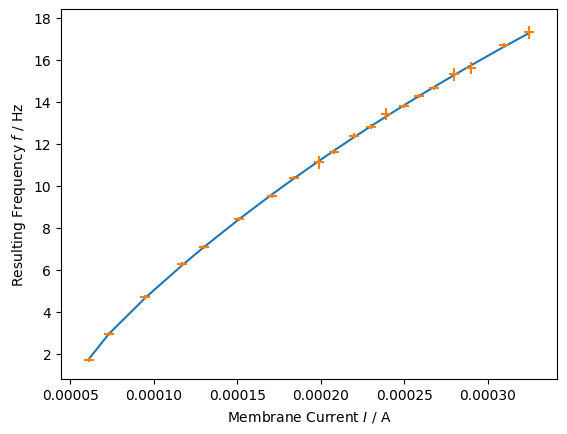
\includegraphics[width=0.5\textwidth]{./Experiments/01_Lui/Graphs/f-I_curve_fitfunc.png}
    \caption{\( f \) - \( I \) Curve of the Lu.i Neuron with Fit Function}
    \label{fig:f-I_curve_fitfunc}
\end{figure}